\documentclass[11pt]{article}

\usepackage[T1]{fontenc}
\usepackage[utf8]{inputenc}
\usepackage[a4paper,left=3.2cm,right=2.4cm,top=2.6cm,bottom=2.6cm]{geometry}
\usepackage{newtxtext}
\usepackage{newtxmath}
\usepackage{microtype}
\usepackage{amsmath,mathtools}
\usepackage{bm}
\usepackage{algorithm}
\usepackage{algpseudocode}
\usepackage{booktabs}
\usepackage{array}
\usepackage{graphicx}
\usepackage{xcolor}
\definecolor{fwblue}{RGB}{31,80,140}
\definecolor{fwgray}{RGB}{95,95,95}
\usepackage{tikz}
\usetikzlibrary{positioning,arrows.meta,fit,backgrounds,calc}
\usepackage{listings}
\usepackage[hidelinks]{hyperref}
\usepackage[round]{natbib}
\bibliographystyle{plainnat}
\usepackage{lineno}
\usepackage[capitalize,noabbrev]{cleveref}

% --- line numbers on the left, WES-style ---
\renewcommand\linenumberfont{\normalfont\tiny\sffamily\color{fwgray}}
\setlength{\parindent}{1.2em}

% --- code listing style for the schedule signature / prompt ---
\lstdefinestyle{fw}{
  basicstyle=\ttfamily\footnotesize,
  breaklines=true,
  columns=fullflexible,
  keepspaces=true,
  showstringspaces=false,
  frame=none,
  xleftmargin=1.2em,
}
\lstset{style=fw}

\newcommand{\gm}{\gamma_{\min}}
\newcommand{\Dmin}{D_{\min}}
\newcommand{\aep}{\mathrm{AEP}}

\title{\vspace{-1.5em}\bfseries\large Scale-Aware Evolutionary Discovery of Wind-Farm\\
Layout Optimizers with Large Language Models}
\author{\normalsize Author One\quad Author Two\quad Author Three\\[0.2em]
\small ADDRESS\\[-0.2em]\small \textit{Correspondence:} (EMAIL)}
\date{}

\begin{document}
\maketitle
\thispagestyle{empty}
\linenumbers

\vspace{-1.2em}
\begin{abstract}
\noindent
We present a framework for the automated discovery of \emph{deployable} learning-rate
and constraint-penalty schedules for gradient-based wind-farm layout optimization
using large language models (LLMs). Candidate schedules are expressed in a
\emph{scale-aware} parameterization in which the exploration learning rate is
constructed from the rotor diameter and the only user-supplied scale is the
constraint tolerance, so a single schedule generalizes across farms of different
size with no free per-farm parameter. An island-based, quality-diversity
evolutionary loop drives LLM coding agents to propose schedules, which a multi-stage
\emph{cascade} evaluator scores across a multi-farm, multi-scale training suite under
a hard feasibility gate. A behavioral archive, content-addressed caching, and
complete lineage provenance make every discovery auditable and, on a fixed platform,
bit-reproducible; a firewall discipline keeps held-out and test performance out of the search. We
describe the schedule interface, the fixed optimization skeleton, the evolutionary
loop and cascade evaluator, the fitness, selection, and deployment rules, and the
reproducibility and firewall machinery that together turn opportunistic program
search into a repeatable engineering procedure.
\end{abstract}

\section{Introduction}
\label{sec:intro}
When designing a wind farm, the placement of turbines within the buildable area
determines every downstream stage of a project, from land valuation to annual
energy production (AEP). Because a fraction-of-a-percent gain in modeled AEP can
translate into a large change in a project's financial case, layout optimization is
a well-studied problem: it is a non-convex, non-linear, constrained optimization in
which turbine positions interact through wake losses and must respect spacing and
boundary (inclusion/exclusion zone) constraints.

Gradient-based solvers have become a de-facto method for this problem. The TopFarm
stochastic gradient descent (SGD) optimizer \citep{quick2023sgd} adapts the Adam
algorithm \citep{kingma2015adam} with a scheduled learning rate and a scheduled
linear constraint penalty. The \emph{schedule} --- how the learning rate, the penalty
weight, and the two Adam moment-decay coefficients evolve over the course of the
optimization --- is a rich design space that governs the trade-off between exploring
the layout and driving the final iterate onto the feasible set. It is precisely the
kind of low-dimensional, high-leverage function that is difficult to design by hand
and attractive to search automatically.

Large language models have recently been used as the mutation operator in
evolutionary \emph{program search}: FunSearch \citep{fawzi2024funsearch} and
AlphaEvolve \citep{deepmind2025alphaevolve} evolve populations of programs by
repeatedly prompting an LLM to improve high-scoring candidates. We adopt this
paradigm for optimizer-schedule design, and add three ingredients that make the
discovered artifact \emph{deployable} rather than merely high-scoring on one farm:

\begin{enumerate}
\itemsep0.15em
\item a \textbf{scale-aware schedule interface} (Section~\ref{sec:interface}) that
removes the free learning-rate parameter and builds the exploration scale from the
rotor diameter, so a discovered schedule is scale-covariant and transfers across
farms of different turbine size;
\item a \textbf{quality-diversity evolutionary loop with a cascade evaluator}
(Sections~\ref{sec:evo}--\ref{sec:cascade}) that scores candidates across a
multi-farm, multi-scale training suite under a hard feasibility gate, rejecting
infeasible or dominated schedules cheaply before spending on expensive high-count
evaluations; and
\item a \textbf{provenance, firewall, and reproducibility layer}
(Sections~\ref{sec:provenance}--\ref{sec:repro}) --- full lineage, a behavioral
archive, content-addressed caching, a scoped mutator workspace, and a pre-registered
selection and deployment criterion --- so that any ``the system discovered $X$''
claim is auditable against what was seeded and what was measured.
\end{enumerate}

The remainder of the paper describes the framework (Section~\ref{sec:framework}),
the wind farms and evaluation cells it is applied to (Section~\ref{sec:application}),
and the reproducibility and cost-control machinery (Section~\ref{sec:repro}).

\section{Framework}
\label{sec:framework}
This section describes the discovery framework: the optimization problem
(\ref{sec:problem}), the scale-aware schedule interface (\ref{sec:interface}), the
fixed optimization skeleton (\ref{sec:skeleton}), the penalty normalization
(\ref{sec:alpha0}), the evolutionary loop (\ref{sec:evo}) and its behavioral archive
(\ref{sec:archive}), the cascade evaluator (\ref{sec:cascade}), the fitness and
feasibility rules (\ref{sec:fitness}), and the provenance, firewall, selection, and
deployment machinery (\ref{sec:provenance}--\ref{sec:selection}). Figure~\ref{fig:loop}
gives the overall data flow.

\subsection{Optimization problem}
\label{sec:problem}
For a farm with $N$ turbines at horizontal positions $(\bm x,\bm y)$ we maximize the
modeled annual energy production
\begin{align}
\max_{\bm x,\bm y}\; J(\bm x,\bm y),\qquad
J = \frac{8760}{10^6}\sum_{k} w_k\, P\!\left(\bm x,\bm y;\,u^{(k)}_\infty,\theta^{(k)}\right),
\label{eq:aep}
\end{align}
where $P$ is the wind-farm power under inflow speed $u^{(k)}_\infty$ and direction
$\theta^{(k)}$ with probability weight $w_k$, evaluated with an engineering wake
model \citep{bastankhah2014wake}, subject to the feasibility constraints
\begin{align}
d(x_i,y_i) \ge 0 \;\;\forall i,\qquad
\sqrt{(x_i-x_j)^2+(y_i-y_j)^2}\ \ge\ \Dmin \;\;\forall i\neq j,
\label{eq:cons}
\end{align}
where $d(x_i,y_i)$ is the signed distance from turbine $i$ to the nearest inclusion-zone
boundary (negative outside the buildable region) and $\Dmin$ is the minimum
inter-turbine spacing. Feasibility is judged against a tolerance $\gm$ (in metres):
a layout is feasible when every turbine satisfies the boundary constraint to within
$\gm$ and the pairwise spacing constraint. $\gm$ is the single user-supplied scale of
the problem.

\subsection{Scale-aware schedule interface}
\label{sec:interface}
The object we search over is a pure function that returns, at each optimization step
$i$, the four quantities the skeleton needs: a learning rate $\eta_i$, a constraint
penalty multiplier $\alpha_i$, and the two Adam moment-decay coefficients
$\beta_{1,i},\beta_{2,i}$:
\begin{align}
\big(\eta_i,\alpha_i,\beta_{1,i},\beta_{2,i}\big)
= \mathcal{S}\big(i,\,T,\,D,\,\Dmin,\,N,\,\gm,\,\alpha_0\big).
\label{eq:schedule}
\end{align}
The arguments are the current step $i$, the total number of steps $T$, and the
\emph{problem-intrinsic scales}: the rotor diameter $D$, the minimum spacing $\Dmin$,
the turbine count $N$, the metre-valued constraint tolerance $\gm$, and a
skeleton-computed penalty normalizer $\alpha_0$ (Section~\ref{sec:alpha0}). The
Python signature is reproduced in Appendix~\ref{app:iface}.

Two design choices make a discovered schedule deployable across scales:

\paragraph{No free learning rate.} There is no driver-supplied initial learning rate
$\eta_0$ anywhere in \cref{eq:schedule}. The exploration scale must be constructed
\emph{inside} the schedule from the rotor diameter, e.g.\ a peak learning rate
$\eta_{\text{peak}} = c\,D$ with $c$ a schedule-internal constant or curve that the
search may evolve but that is never a user knob. Because the turbine spacing, wake
length, and feasible-region geometry all scale with $D$, expressing the exploration
scale as a multiple of $D$ makes the schedule scale-covariant: the same function
applied to a farm with a different rotor diameter automatically takes appropriately
sized steps.

\paragraph{Tolerance as the terminal learning rate.} Following TopFarm's own
convention, the terminal learning rate is a proxy for how tightly the boundary is
ultimately satisfied; we expose it directly as the metre-valued tolerance $\gm$
toward which the schedule decays the learning rate. It is the only user-supplied
scale, and a faithful schedule must respond to it: at a looser $\gm$ the schedule
should stop decaying sooner, and its terminal behavior and feasibility should change
accordingly (this responsiveness is checked in Section~\ref{sec:cascade}).

\subsection{Fixed optimization skeleton}
\label{sec:skeleton}
The schedule is the \emph{only} thing the search controls. A fixed skeleton
(Algorithm~\ref{alg:skeleton}) handles initialization, gradient computation, and the
Adam update. It (i)~places the initial layout on a wind-direction-aware grid inside
the buildable region (for the multi-zone case, on a zone-interior fill); (ii)~forms
the objective gradient of \cref{eq:aep} and the constraint gradient of the boundary
and spacing penalties by automatic differentiation; (iii)~combines them as
$\bm j = \nabla_{\!\text{obj}} + \alpha_i\,\nabla_{\!\text{con}}$; and (iv)~applies an
Adam step with the scheduled $\eta_i,\beta_{1,i},\beta_{2,i}$. The horizon is fixed at
$T=8000$ steps. Nothing in the skeleton contains a hardcoded learning rate; the entire
step-size behavior comes from \cref{eq:schedule}.

\begin{algorithm}[t]
\caption{Fixed optimization skeleton (the search controls only $\mathcal{S}$)}
\label{alg:skeleton}
\begin{algorithmic}[1]
\State $\bm s \gets \text{wind-aware init}(D,\Dmin,N,\text{resource})$;\quad
       $\bm m,\bm v \gets \bm 0$
\State $\alpha_0 \gets \operatorname{mean}\!\big(|\nabla_{\!\bm s}J(\bm s)|\big)/D$;\quad
       $\alpha_0 \gets \textsc{canonicalize}(\alpha_0)$ \Comment{Section~\ref{sec:alpha0}}
\For{$i = 0,1,\dots,T-1$}
  \State $(\eta_i,\alpha_i,\beta_{1,i},\beta_{2,i}) \gets
          \mathcal{S}(i,T,D,\Dmin,N,\gm,\alpha_0)$
  \State $\bm j \gets \nabla_{\!\bm s}\big[-J(\bm s)\big] \;+\; \alpha_i\,\nabla_{\!\bm s}\,\gamma(\bm s)$
         \Comment{objective $+$ penalty gradient}
  \State $\bm m \gets \beta_{1,i}\bm m + (1-\beta_{1,i})\bm j$;\quad
         $\bm v \gets \beta_{2,i}\bm v + (1-\beta_{2,i})\bm j^2$
  \State $\hat{\bm m}\gets \bm m/(1-\beta_{1,i}^{\,i+1})$;\quad
         $\hat{\bm v}\gets \bm v/(1-\beta_{2,i}^{\,i+1})$
  \State $\bm s \gets \bm s - \eta_i\,\hat{\bm m}/\sqrt{\hat{\bm v}}$
\EndFor
\State \Return $\bm s$
\end{algorithmic}
\end{algorithm}

\subsection{Penalty normalization}
\label{sec:alpha0}
So that the penalty multiplier is on a problem-intrinsic scale, the skeleton computes
the normalizer
\begin{align}
\alpha_0 = \frac{\operatorname{mean}\big(|\nabla_{\!\bm x}J|,\,|\nabla_{\!\bm y}J|\big)}{D}
\label{eq:alpha0}
\end{align}
at the initial layout and passes it into \cref{eq:schedule}; the schedule composes the
running penalty $\alpha_i$ from $\alpha_0$. Normalizing the gradient magnitude by the
rotor diameter (rather than by a learning rate) keeps the penalty scale covariant with
the geometry and independent of the step-size choice, consistent with the removal of a
free learning rate. To make evaluation bit-reproducible across \emph{independent
processes on a given platform}, $\alpha_0$ is canonicalized to single precision at the
skeleton boundary (\textsc{canonicalize} in Algorithm~\ref{alg:skeleton}): the
double-precision gradient reduction agrees to far more significant figures than single
precision, so rounding $\alpha_0$ to a canonical single-precision value makes the same
$(\text{schedule},\text{cell},\text{seed})$ reproduce identically in independent
processes. This matters because the low--learning-rate tail of the optimization is
sensitive to $\alpha_0$. Across \emph{different} hardware architectures a small
floating-point drift remains; we therefore report cross-platform agreement to within a
measured drift tolerance (Section~\ref{sec:repro}) rather than bit-identity.

\subsection{Evolutionary discovery loop}
\label{sec:evo}
Schedules are discovered by a quality-diversity evolutionary loop
(Algorithm~\ref{alg:evo}), built on an island model with a MAP-Elites archive
\citep{mouret2015mapelites} per island. Each iteration: (i)~a parent schedule is
sampled from an island's archive with a fitness- and novelty-aware sampler; (ii)~an
LLM mutation engine is prompted with the parent source and firewall-safe feedback and
returns an improved schedule as Python source; (iii)~a code-novelty filter rejects a
child that is a near-duplicate of an already-seen program before any expensive
evaluation is spent; (iv)~the survivor is scored by the cascade evaluator
(Section~\ref{sec:cascade}); and (v)~it is inserted into the island's behavioral
archive if it is elite for its cell. Islands periodically exchange elites. The loop
runs until a token/cost ceiling is reached (Section~\ref{sec:repro}).

The population is \emph{seeded} with known-good schedules, logged as generation-0
ancestors with their port transforms (Section~\ref{sec:provenance}); the search is an
engineering procedure and seeding is encouraged. The mutation operators are LLM coding
agents accessed through a subscription/OAuth path (the Claude Agent SDK is the primary
engine; a command-line Gemini engine and a deterministic mock engine are also
supported). We adopt two eval-saving mechanisms from ShinkaEvolve
\citep{shinka2025}: code-novelty rejection-sampling and fitness/novelty-aware parent
sampling; the island/MAP-Elites and cascade scaffolding follow OpenEvolve
\citep{openevolve2025}.

\begin{algorithm}[t]
\caption{Evolutionary schedule discovery}
\label{alg:evo}
\begin{algorithmic}[1]
\State seed each island archive with generation-0 ancestors (logged with lineage)
\While{cost $<$ ceiling}
  \For{each island}
    \State $p \gets$ \textsc{SampleParent}(archive) \Comment{fitness/novelty-aware}
    \State materialize a scoped mutator workspace (Section~\ref{sec:firewall})
    \State $c \gets$ \textsc{LLM-Mutate}$(p,\ \text{firewall-safe feedback})$
    \If{\textsc{NoveltyFilter} rejects $c$} \textbf{continue} \EndIf
    \State $(\text{fit}, \text{feasible}, \text{desc}) \gets$ \textsc{Cascade}$(c)$
           \Comment{Algorithm/Section~\ref{sec:cascade}}
    \If{feasible} \textsc{ArchiveInsert}(island, $c$, fit, desc) \EndIf
    \State \textsc{LogLineage}$(c, p, \text{engine}, \text{tokens}, \text{cost}, \text{desc}, \text{fit})$
  \EndFor
  \State periodically migrate elites between islands; checkpoint state
\EndWhile
\end{algorithmic}
\end{algorithm}

\subsection{Behavioral archive}
\label{sec:archive}
Each candidate is placed in a MAP-Elites archive keyed by four behavioral descriptors
computed from the schedule function \emph{before} evaluation, so that the archive
covers qualitatively distinct schedule shapes rather than crowding a single family
(Table~\ref{tab:bins}): the peak learning rate relative to the rotor diameter, the
terminal learning rate in metres, the coupling between the penalty and the learning
rate, and the number of learning-rate restarts. Within each island, one elite is kept
per occupied cell; feasibility dominates, then mean fitness, then a worst-cell
tiebreak (Section~\ref{sec:fitness}). Seeding populates several descriptor cells from
generation~0.

\begin{table}[t]
\centering
\small
\caption{Behavioral descriptors and their (frozen) bins for the MAP-Elites archive.
Descriptors are computed from the schedule function prior to evaluation.}
\label{tab:bins}
\begin{tabular}{@{}ll@{}}
\toprule
Descriptor & Bins \\
\midrule
Peak learning rate $/\,D$ & $<0.5,\ \ 0.5\text{--}0.8,\ \ 0.8\text{--}1.2,\ \ {>}1.2$ \\
Terminal learning rate (m) & $\le 0.01,\ \ 0.01\text{--}0.1,\ \ 0.1\text{--}1,\ \ {>}1$ \\
Penalty coupling & coupled,\ \ decoupled,\ \ cyclic \\
Learning-rate restarts & $0,\ \ 1\text{--}2,\ \ \ge 3$ \\
\bottomrule
\end{tabular}
\end{table}

\subsection{Cascade evaluator}
\label{sec:cascade}
Evaluating a schedule on every training cell at full seed count is expensive, so
candidates pass through a cascade that spends compute in proportion to promise. Each
stage runs the fixed skeleton (Algorithm~\ref{alg:skeleton}) on a cell/seed and
records the resulting AEP and feasibility.

\begin{description}
\itemsep0.2em
\item[Stage A (gross fast-reject).] Two cheap cells $\times$ two seeds. This is a
deliberately \emph{gross} filter: a candidate is rejected only if any seed is
infeasible or its AEP is more than about one percent below that cell's reference. It is
\emph{not} texture-floor-tight --- a floor-tight Stage~A would mass-reject the very
exploration the quality-diversity archive exists to keep, so the texture floors are
reserved for selection margins, not for this filter. The rejection rate by cause
(infeasible vs.\ below-reference) is logged as a pilot diagnostic. No high-count cell is
used here.
\item[Stage B (training matrix).] The full frozen training set (Table~\ref{tab:cells})
$\times$ at least five \emph{paired} seeds --- the same seed produces the same
wind-aware initial layout for the candidate and for the reference, so per-seed
differences are paired. Each cell yields a percentage score (Section~\ref{sec:fitness})
and a candidate-feasibility flag; the cross-cell aggregate is the candidate's stage-B
fitness.
\item[Stage B$^{+}$ (elite tier).] Top-$k$ archive elites are re-scored on expensive
high-count cells, where a longer per-evaluation budget is affordable. This stage runs
only on dedicated compute and never inside the main loop. It also carries the
\emph{capability-frontier} cells --- cells (a high-count single-polygon farm and a
dense multi-zone farm under a unidirectional resource) on which even the reference
schedule is infeasible. These are tracked at the elite tier as qualitative probes: a
candidate that reaches strict feasibility there is a qualitatively new result. They
never gate the per-generation search; off the dedicated compute they are simply marked
pending and deferred.
\item[Stage C (holdout \& responsiveness).] Elites are scored on the held-out farm for
margin-aware selection (Section~\ref{sec:selection}) and are re-scored at a looser
tolerance to confirm the schedule \emph{responds} to $\gm$ (feasibility and terminal
behavior must change); a schedule invariant to the tolerance is rejected regardless of
AEP. The held-out AEP never leaves this stage: only feasibility booleans and a
margin-over-floor boolean cross the firewall (Section~\ref{sec:firewall}).
\end{description}

\subsection{Fitness and feasibility}
\label{sec:fitness}
For a training cell $c$, over the shared paired seed set, the score is the percentage
improvement in mean AEP over a reference schedule,
\begin{align}
\text{score}_c \;=\; 100\times
\frac{\overline{\aep}_{\text{cand},c}-\overline{\aep}_{\text{ref},c}}{\overline{\aep}_{\text{ref},c}},
\label{eq:score}
\end{align}
where the reference is the native TopFarm monotone schedule at a rotor-diameter-scaled
learning rate, $\eta_{\text{peak}}=c_0 D$ with $c_0$ calibrated once on the training
farm, decaying to $\gm$. Expressing fitness as percent-over-reference makes cells of
very different magnitude (thousands of GWh for the large offshore farms, hundreds for
the small onshore multi-zone farm) commensurable. The reference AEP
$\overline{\aep}_{\text{ref},c}$ is used purely as a \emph{scale constant}: it
normalizes the candidate even on a cell where the reference itself is infeasible, and
the reference's feasibility never confers credit.

Feasibility at $\gm$ is a \emph{hard gate}: a candidate must be feasible on every
paired seed of every training cell, or it is rejected (its score is set to $-\infty$
and it is excluded from the archive as infeasible). The cross-cell aggregate is
\emph{farm-balanced}: the mean over farms of each farm's mean cell score, with a
worst-cell tiebreak,
\begin{align}
\text{fitness} \;=\;
\frac{1}{|\mathcal{F}|}\sum_{f\in\mathcal{F}}
\frac{1}{|\mathcal{C}_f|}\sum_{c\in\mathcal{C}_f}\text{score}_c,
\qquad
\text{tiebreak} \;=\; \min_{c}\text{score}_c,
\label{eq:agg}
\end{align}
where $\mathcal{F}$ is the set of farms and $\mathcal{C}_f$ the scored cells on farm
$f$. Averaging over farms rather than over cells makes each farm contribute equally
irrespective of how many cells it carries (the training set has more cells on the
large offshore farm than on the small multi-zone farm), so a percent improvement is
worth the same on either farm; the worst-cell tiebreak still prevents a large win on
one easy cell from masking a regression on a hard one. The aggregate is taken over the
\emph{scored} cells. A cell whose objective is saturated --- for example a
unidirectional resource in which every constraint-feasible layout that separates the
turbines reaches free-stream power, so all such layouts score identically --- carries
no AEP-improvement signal; it is retained as a \emph{feasibility-only} gate (evaluated
at two seeds, participating in the hard feasibility gate) but is excluded from the
scored set.

\subsection{Provenance and lineage}
\label{sec:provenance}
Every candidate is recorded in an append-only lineage log with a content hash, its
parent identifier(s), the mutation engine and model string, the token count and
monetary cost, its behavioral descriptors, its per-cell fitness, and its generation
and island. Seeded ancestors are logged as generation~0 together with their port
transforms. Because the seeds and their transforms are recorded, any later claim that
the system \emph{discovered} a schedule family is measured against what was seeded, and
``discovered'' is distinguishable from ``recombined a seed.''

\subsection{Firewall and scoped workspace}
\label{sec:firewall}
The search must not overfit to, or leak, the held-out and test farms. Two disciplines
enforce this. First, \emph{information firewall}: only firewall-safe feedback ---
per-cell percentage scores and feasibility booleans --- ever reaches a mutation
engine; held-out and test AEP values never enter a mutator's context or transcript,
and the pre-registration of the selection and test design (Section~\ref{sec:selection})
lives outside the search entirely. Second, \emph{workspace scoping}: before each
mutation the engine is run inside a freshly materialized clean-room directory that
contains only the schedule interface, a sanitized copy of the skeleton and seed
schedules, and the firewall-safe feedback; the results, analysis, held-out state, and
pre-registration are outside the engine's working directory and tool scope.
Sanitization strips provenance and redacts any residual path token from the reference
code, and a gate check refuses to launch if a forbidden token or a syntactically
invalid reference file is present in the scoped workspace.

\subsection{Selection and deployment criterion}
\label{sec:selection}
Selection is margin-aware and never a single-evaluation argmax. Among the archive
elites that are feasible on the training and held-out farms, the deployed schedule is
the one that maximizes the multi-seed validation-mean margin over the reference on the
held-out farm, provided that margin exceeds the held-out cell's evaluation-texture
floor; if no elite clears the margin, the native seed is deployed and the run is
recorded as producing no improvement. The deployment claim is then confirmed, once, on
a pre-registered test set under a paired multi-seed protocol (identical per-seed
initial layouts across arms) and, as a fidelity stage, re-validated in the full
stochastic optimizer. Because feasibility is judged against a tolerance and reference
results depend on it, all comparisons are reported at matched tolerance.

\begin{figure}[t]
\centering
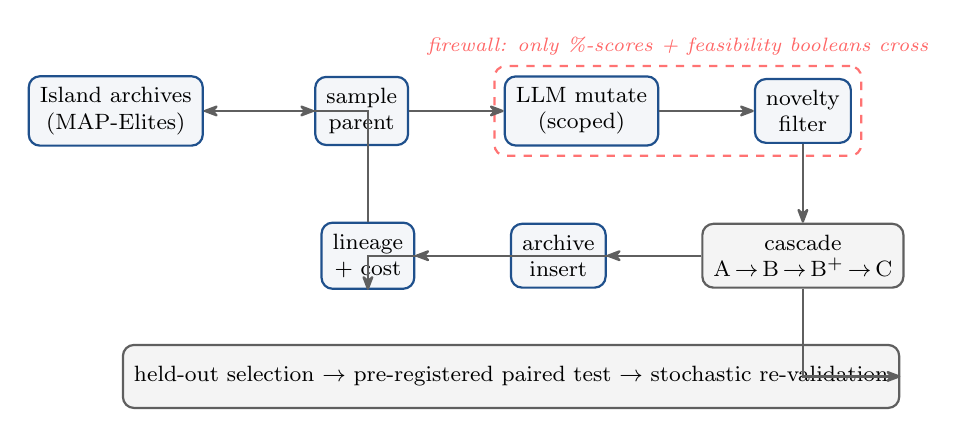
\begin{tikzpicture}[
  font=\footnotesize,
  >={Stealth[round]},
  box/.style={draw=fwblue,thick,rounded corners,align=center,inner sep=4pt,fill=fwblue!5,minimum height=8mm},
  cbox/.style={draw=fwgray,thick,rounded corners,align=center,inner sep=4pt,fill=fwgray!7,minimum height=8mm},
  ar/.style={->,thick,fwgray},
]
\node[box] (arch) {Island archives\\(MAP-Elites)};
\node[box,right=14mm of arch] (samp) {sample\\parent};
\node[box,right=12mm of samp] (mut) {LLM mutate\\(scoped)};
\node[box,right=12mm of mut] (nov) {novelty\\filter};
\node[cbox,below=10mm of nov] (cas) {cascade\\A\,$\to$\,B\,$\to$\,B$^+$\,$\to$\,C};
\node[box,left=12mm of cas] (ins) {archive\\insert};
\node[box,left=12mm of ins] (log) {lineage\\+ cost};

\draw[ar] (arch) -- (samp);
\draw[ar] (samp) -- (mut);
\draw[ar] (mut) -- (nov);
\draw[ar] (nov) -- (cas);
\draw[ar] (cas) -- (ins);
\draw[ar] (ins) -- (log);
\draw[ar] (log) |- (arch);
\draw[ar] (cas.west) -- ++(-0.0,0) -| (log.south);

% firewall band around the mutation region
\begin{scope}[on background layer]
  \node[draw=red!55,dashed,thick,rounded corners,fit=(mut)(nov),
        label={[red!60,font=\scriptsize\itshape]above:firewall: only \%-scores + feasibility booleans cross}] {};
\end{scope}

\node[cbox,below=7mm of ins,xshift=-6mm] (sel) {held-out selection $\rightarrow$ pre-registered paired test $\rightarrow$ stochastic re-validation};
\draw[ar] (cas.south) |- (sel.east);
\end{tikzpicture}
\caption{The discovery loop. Parents are sampled from per-island MAP-Elites archives;
an LLM mutation engine, run inside a scoped clean-room workspace, proposes a child
schedule from the parent source and firewall-safe feedback; a novelty filter rejects
near-duplicates before evaluation; the cascade evaluator scores survivors; feasible
elites are archived and every candidate is logged with full provenance. Held-out
selection, the pre-registered paired test, and stochastic re-validation sit outside
the loop.}
\label{fig:loop}
\end{figure}

\section{Application}
\label{sec:application}
We apply the framework across three wind-farm geometries and four wind resources. The
farms span a range of rotor diameters and constraint geometries: the Danish Energy
Island (DEI) cluster with IEA 15\,MW turbines ($D=240$\,m, single polygon); the IEA
Wind 740-10-MW Reference Offshore Wind Plant (ROWP) with IEA 10\,MW turbines
($D=198$\,m, single polygon), held out for selection; and the Parque Ficticio
inclusion-zone case of \citet{criadorisco2024} with Vestas V80 turbines ($D=80$\,m,
five disconnected inclusion zones --- the hardest feasibility geometry). Minimum
spacing is four rotor diameters for DEI and ROWP and two rotor diameters for Parque.
We consider four wind resources: the measured DEI and ROWP roses, an omnidirectional
resource, and a unidirectional resource as limiting cases.

\paragraph{Training cells.} The search optimizes and sees percentage feedback on the
training cells of Table~\ref{tab:cells}, which span two rotor diameters, turbine counts
from 10 to 120, three resource types (the DEI rose, omnidirectional, and unidirectional
--- the ROWP rose is held out), the multi-zone geometry, and a high-count cell. Two
cheap cells serve as the Stage-A fast-reject filter. The reference AEP column is the
scale constant of \cref{eq:score}, and the floor column is the per-cell texture floor.
One Parque cell under the unidirectional resource is a feasibility-only gate: its
objective is saturated (Section~\ref{sec:fitness}), so it is scored for feasibility only
and excluded from the aggregate. The two capability-frontier cells
(Section~\ref{sec:cascade}) --- a high-count DEI cell and a dense Parque cell under the
unidirectional resource, on which even the reference is infeasible --- are not training
cells; they are elite-tier probes only.

\begin{table}[t]
\centering
\small
\caption{Training cells (all references feasible on every seed). $D$ in metres; Ref.\
AEP is the rotor-diameter-scaled reference (the scale constant of \cref{eq:score}), a
multi-seed feasible mean in GWh; Floor is the per-cell evaluation-texture floor (GWh).
``feas.-only'' marks the saturated-objective cell that gates feasibility but is excluded
from the score aggregate.}
\label{tab:cells}
\begin{tabular}{@{}llrrlrr@{}}
\toprule
Cell & Farm & $N$ & $D$ & Resource & Ref.\ AEP & Floor \\
\midrule
DEI-50            & DEI    & 50  & 240 & DEI rose        & 5560.4  & 0.3 \\
DEI-80            & DEI    & 80  & 240 & omnidirectional & 8818.1  & 0.3 \\
DEI-120           & DEI    & 120 & 240 & DEI rose        & 13030.0 & 0.3 \\
DEI-50 uni.       & DEI    & 50  & 240 & unidirectional  & 5598.4  & 0.3 \\
Parque-20         & Parque & 20  & 80  & DEI rose        & 231.5   & 0.1 \\
Parque-14 uni.    & Parque & 14  & 80  & unidirectional  & \textit{184.8 (f.o.)} & 0.1 \\
Parque-10         & Parque & 10  & 80  & omnidirectional & 127.0   & 0.1 \\
\bottomrule
\end{tabular}
\end{table}

\paragraph{Held-out and test farms.} ROWP is an intermediate scale not present in
training and is used only for margin-aware selection; its AEP is firewalled from the
search. The pre-registered test set --- touched exactly once, at the deployment
decision --- comprises the high-count ROWP cells ($N=200$ and $N=300$), the Parque
site's real heterogeneous wind resource, and a unidirectional extreme on the held-out
ROWP farm.

\paragraph{Evaluation-texture floors.} AEP is a mildly discontinuous function of the
layout because the wake model masks each turbine's contribution outside a cone; at
millimetre-scale perturbations this yields a small texture in re-scored AEP. We measure
this floor per farm and set the per-cell minimum meaningful margin accordingly:
$0.3$\,GWh for the large offshore DEI farm, $0.1$\,GWh for the multi-zone Parque farm,
and $0.64$\,GWh for the held-out ROWP farm. Selection margins use these per-cell floors
rather than a single global threshold; the gross Stage-A filter
(Section~\ref{sec:cascade}) does not use them.

\subsection{Reference multistart budget and its convergence}
\label{sec:convergence}
The score of \cref{eq:score} compares a candidate against a single reference run per
seed, but the baseline a \emph{deployed} schedule must actually beat is stronger: the
best feasible layout a practitioner would field from a \emph{multistart} of $K$
independent random initializations of the reference. The number of starts that defines a
converged multistart is not arbitrary; we fix it per farm with the shuffle-saturation
analysis of \citet{quick2026neighbors}. A pool of $M$ feasible reference runs is
collected on a farm; the pool is randomly reshuffled $10^3$ times, and for each shuffle
the running maximum AEP is recorded against the number of starts considered. The $p$-th
percentile of that running maximum across shuffles is a conservative estimate of the best
AEP obtained with that many starts --- the first percentile is the value beaten $99\%$ of
the time --- and the convergence budget $K^\star$ is the number of starts at which that
percentile reaches within a tolerance of the pool maximum (made precise below). The pool
is large enough to resolve $K^\star$ when $K^\star\le M/2$; otherwise the pool is doubled
and the analysis repeated.

Because AEP is effectively continuous near the optimum, the single best run of a pool is
an isolated point, so reaching the \emph{exact} pool maximum saturates only at
$\approx0.99\,M$ regardless of $M$. We therefore read saturation at a physically
negligible tolerance $\epsilon$ (reaching within $\epsilon$ of the pool maximum) and
report $K^\star$ across $\epsilon$. The budget is then a property of the density of the
near-optimum basin: if a fraction $f_\epsilon$ of runs land within $\epsilon$ of the
best, the first-percentile budget approaches $\ln(0.01)/\ln(1-f_\epsilon)$ as the pool
grows.

We calibrate on the DEI training farm and the held-out ROWP farm with pools of
$M\!\approx\!4000$ feasible reference runs each, collected as HPC array jobs
(\cref{fig:convergence,tab:convergence}). The per-pool convergence estimate is itself
noisy at small pools --- on the held-out farm the first-percentile budget is
$420\pm214$ at $M=1024$ against $\approx\!1086$ at the deep pool --- so it is the deep
pools with $10^3$-shuffle averaging, not a single half-pool check, that make $K^\star$
trustworthy; at the deep pools the half-pool rule holds on both farms
($K^\star_1\le M/2$), confirming the pool is large enough to resolve the budget. ROWP is
consistently the harder farm: its near-optimum basin is sparser ($0.39\%$ of runs within
$0.05\%$ of the best against $0.52\%$ for DEI, and $3.5\%$ vs.\ $9.3\%$ within $0.1\%$),
so it requires $1.3$--$3\times$ more starts than the training farm. At the tenth
percentile the budget is $\approx\!290$ starts for DEI and $\approx\!550$ for ROWP; for
first-percentile confidence within $0.05\%$ of the optimum it is $\approx\!520$ and
$\approx\!1090$ (asymptotically $\approx\!880$ and $\approx\!1180$). The $400$-start
choice of \citet{quick2026neighbors} for their DEI farm falls between our tenth- and
first-percentile DEI budgets, consistent with this calibration.

We adopt a reference multistart of $K=1024$ starts. This exceeds the first-percentile
budget on the training farm and the fifth-percentile budget on the held-out farm
($K^\star_5\approx730$), and covers the held-out first percentile at the $0.1\%$
tolerance ($\approx\!130$); at the strictest $0.05\%$ tolerance it sits just below the
held-out first-percentile budget ($\approx\!1086$), a shortfall we regard as immaterial
at that margin. Deployment comparisons (\cref{sec:selection}) are made against the
best-of-$K$ of this multistart at matched start count, not against its mean.

\begin{figure}[t]
\centering
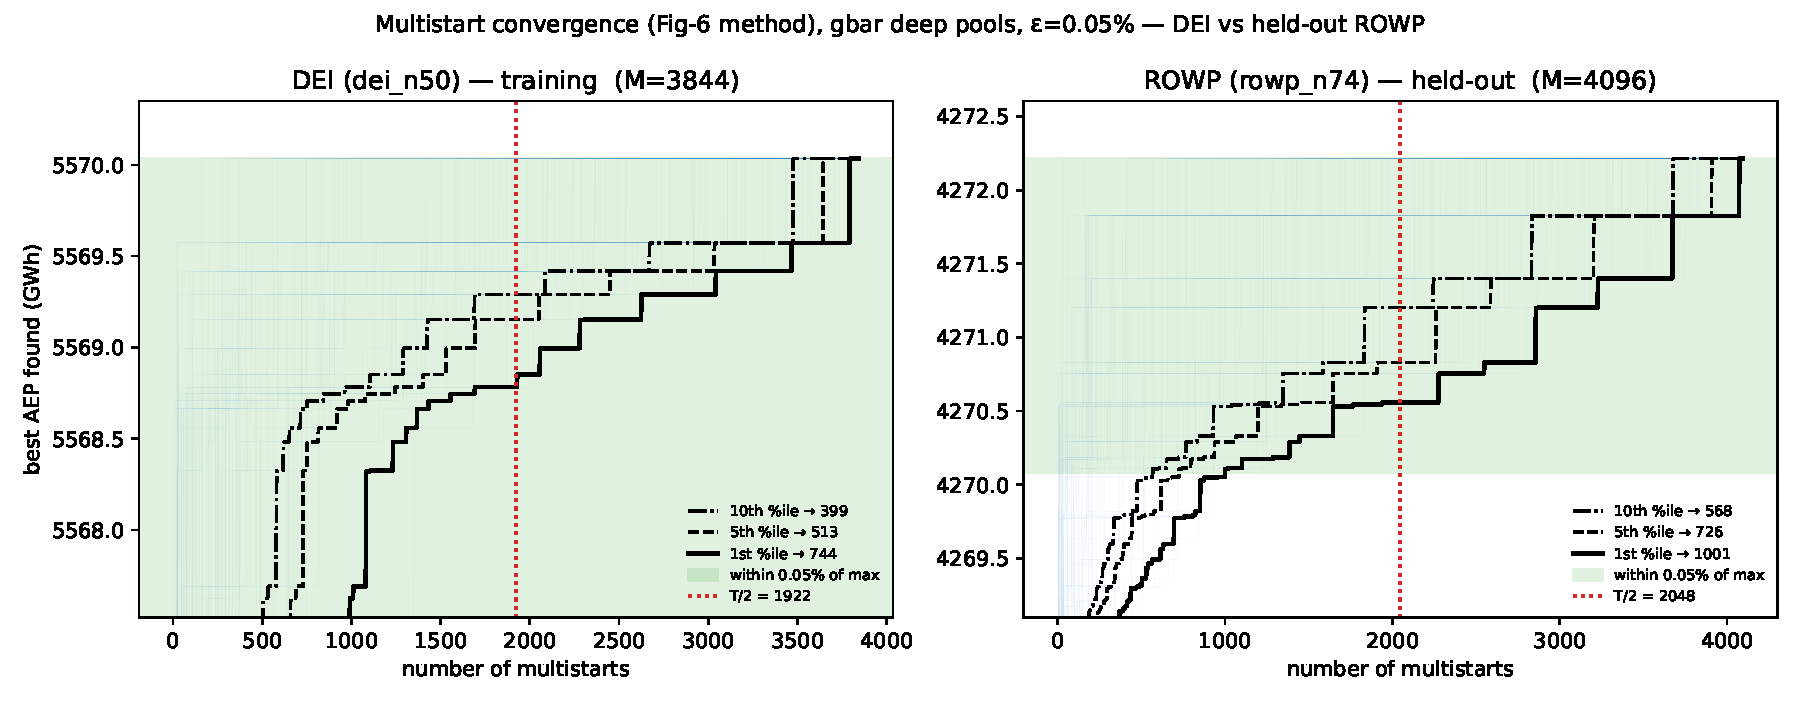
\includegraphics[width=\linewidth]{fig_convergence.pdf}
\caption{Shuffle-saturation convergence of the reference multistart on the DEI training
farm (left) and the held-out ROWP farm (right), following \citet{quick2026neighbors}.
Faint lines are individual shuffles of the pool; the black curves are the tenth-, fifth-,
and first-percentile running maxima; the shaded band is within $\epsilon=0.05\%$ of the
pool maximum, and the dotted vertical line is the half-pool budget $M/2$. Each
percentile reaches the band well inside $M/2$ on both farms; the held-out ROWP farm
(sparser near-optimum basin) requires more starts than the training farm.}
\label{fig:convergence}
\end{figure}

\begin{table}[t]
\centering
\small
\caption{Reference-multistart convergence budget per farm. The feasible pool has
$M\!\approx\!4000$ runs (DEI budgets resolved on a $T{=}2048$ sub-pool, ROWP on the full
$T{=}4096$ pool); ``spread'' is the relative AEP range $(\max-\min)/\max$ over the pool;
$f_\epsilon$ is the fraction of runs within $\epsilon$ of the pool maximum; $K^\star_p$
is the pool-measured number of starts at which the $p$-th-percentile running maximum
reaches within $\epsilon$ of the pool maximum. The held-out ROWP farm needs
$1.3$--$3\times$ more starts than the DEI training farm.}
\label{tab:convergence}
\begin{tabular}{@{}lrrrrrr@{}}
\toprule
& spread & $f_{0.05\%}$ & $f_{0.1\%}$ & $K^\star_{10}$ & $K^\star_{1}$ & $K^\star_{1}$ \\
Farm & (\%) & (\%) & (\%) & ($0.05\%$) & ($0.05\%$) & ($0.1\%$) \\
\midrule
DEI-50 (training) & 0.282 & 0.52 & 9.3 & 290 & 520 & 47 \\
ROWP (held-out)   & 0.456 & 0.39 & 3.5 & 546 & 1086 & 130 \\
\bottomrule
\end{tabular}
\end{table}

\section{Reproducibility and cost control}
\label{sec:repro}
The framework is engineered to be re-runnable and auditable. A content-addressed cache
keyed by $(\text{schedule hash},\text{cell},\text{seed},\gm,T)$ returns a stored result
for any previously computed evaluation, so a resumed run recomputes nothing. State ---
the archives, the novelty seen-set, the cost tally, and the generation counter --- is
checkpointed atomically each generation; the parent-sampling randomness is derived from
the run identifier and generation, and parent lists are ordered canonically, so a
resumed run reproduces the same candidates and hits the cache for every evaluation. The
single-precision canonicalization of $\alpha_0$ (Section~\ref{sec:alpha0}) makes each
evaluation \emph{bit-identical across independent processes on a fixed platform}. Across
different hardware architectures a small floating-point drift remains --- of order
$\pm1.7$\,GWh on the large offshore farm between arm64 and x86 in our measurements ---
so cross-platform results are compared at that measured drift tolerance rather than as
bit-identity. A cost ceiling tracks cumulative tokens and spend from the per-invocation
engine logs and cleanly aborts the run near the ceiling (it stops issuing new mutations,
finishes in-flight work, checkpoints, and stops). Together these make a discovery run a
deterministic function of its seeds, configuration, and budget on a fixed platform.

\section{Conclusions}
\label{sec:conclusions}
We described a framework for discovering deployable wind-farm layout optimizers with
large language models. Its distinguishing features are a scale-aware schedule
interface that removes the free learning rate and builds the exploration scale from the
rotor diameter; a quality-diversity evolutionary loop whose cascade evaluator scores
candidates across a multi-farm, multi-scale training suite under a hard feasibility
gate; and a provenance, firewall, and reproducibility layer --- lineage, a behavioral
archive, content-addressed caching, a scoped mutator workspace, and a pre-registered
selection and deployment criterion --- that make the procedure auditable and
repeatable. The framework turns LLM-driven program search from an opportunistic
experiment into an engineering procedure whose output is a schedule ready to be
deployed and confirmed on unseen farms.

\appendix
\section{Schedule interface and mutation prompt}
\label{app:iface}
The searched object is a single Python function; the skeleton, seeds, and firewall-safe
feedback are provided read-only in the scoped workspace.

\begin{lstlisting}
def schedule_fn(step, total_steps, D, min_spacing,
                n_turbines, gamma_min, alpha0):
    """Return (lr, alpha, beta1, beta2) at `step`.

    D          : rotor diameter (m)            -- exploration-scale source
    min_spacing: minimum inter-turbine spacing (m)
    n_turbines : N                             -- density / packing signal
    gamma_min  : constraint tolerance (m)      -- the terminal learning rate,
                                                  the only user-supplied scale
    alpha0     : penalty normalizer = mean(|grad J|)/D  (skeleton-computed)
    """
    ...
    return lr, alpha, beta1, beta2
\end{lstlisting}

\noindent The mutation engine receives, in its scoped workspace: the interface above,
a sanitized copy of the fixed skeleton and the seed schedules, the parent schedule
source, and the firewall-safe feedback (per-cell percentage scores and feasibility
booleans). It returns one improved module defining \texttt{schedule\_fn}. No held-out
or test AEP, and none of the analysis or pre-registration, is ever placed in that
workspace.

\begin{thebibliography}{99}
\small
\bibitem[Bastankhah and Port\'e-Agel(2014)]{bastankhah2014wake}
Bastankhah, M.\ and Port\'e-Agel, F.: A new analytical model for wind-turbine wakes,
\textit{Renewable Energy}, 70, 116--123, 2014.

\bibitem[Criado Risco et al.(2024)]{criadorisco2024}
Criado Risco, J., Valotta Rodrigues, R., Friis-M{\o}ller, M., Quick, J.,
M{\o}lgaard Pedersen, M., and R\'ethor\'e, P.-E.: Gradient-based wind farm layout
optimization with inclusion and exclusion zones, \textit{Wind Energy Science}, 9,
585--600, 2024.

\bibitem[Google DeepMind(2025)]{deepmind2025alphaevolve}
Google DeepMind: AlphaEvolve: a coding agent for scientific and algorithmic discovery,
Technical report, 2025.

\bibitem[Kingma and Ba(2015)]{kingma2015adam}
Kingma, D.\ P.\ and Ba, J.: Adam: a method for stochastic optimization, in
\textit{International Conference on Learning Representations}, 2015.

\bibitem[Mouret and Clune(2015)]{mouret2015mapelites}
Mouret, J.-B.\ and Clune, J.: Illuminating search spaces by mapping elites, arXiv
preprint arXiv:1504.04909, 2015.

\bibitem[OpenEvolve(2025)]{openevolve2025}
OpenEvolve: an open-source evolutionary coding framework, software, 2025.

\bibitem[Quick et al.(2022)]{quick2023sgd}
Quick, J., R\'ethor\'e, P.-E., M{\o}lgaard Pedersen, M., and Rodrigues, R.\ V.:
Stochastic gradient descent for wind farm optimization, \textit{Wind Energy Science
Discussions}, 1--17, 2022.

\bibitem[Quick et al.(2026)]{quick2026neighbors}
Quick, J., R\'ethor\'e, P.-E., Maak, L., and Maheshwari, P.: Wind farm design under
uncertainty: managing unknown neighboring farm effects, in \textit{Proceedings of the
ASME 2026 45th International Conference on Ocean, Offshore and Arctic Engineering
(OMAE)}, OMAE2026-176207, 2026.

\bibitem[Romera-Paredes et al.(2024)]{fawzi2024funsearch}
Romera-Paredes, B., Barekatain, M., Novikov, A., Balog, M., Kumar, M.\ P., Dupont, E.,
Ruiz, F.\ J., Ellenberg, J.\ S., Wang, P., Fawzi, O., et al.: Mathematical discoveries
from program search with large language models, \textit{Nature}, 625, 468--475, 2024.

\bibitem[Sakana AI(2025)]{shinka2025}
Sakana AI: ShinkaEvolve: sample-efficient evolutionary program search with large
language models, software/technical report, 2025.
\end{thebibliography}

\end{document}
